% généré depuis source/05_donnees.md — ne pas modifier à la main
\chapter{Données}\label{sec:donnees}

\chapintro

Ce chapitre décrit le jeu de données C-MAPSS FD001 : son origine, sa structure et ses tailles exactes, le traitement des moteurs encore en service par la censure à droite, et l'analyse exploratoire des capteurs.

\section{Origine et protocole de simulation}\label{sec:donnees-origine}

Les données proviennent du simulateur C-MAPSS (\emph{Commercial Modular Aero-Propulsion System Simulation}) de la NASA \cite{saxena2008damage}. Chaque moteur démarre avec un niveau d'usure initial et une dispersion de fabrication inconnus, considérés comme normaux. Au cours des cycles de vol, une dégradation est injectée dans le compresseur haute pression (HPC) jusqu'à la défaillance, définie par le franchissement d'une marge de fonctionnement. Les mesures sont bruitées. Le sous-ensemble FD001 retenu ici est le plus simple : \textbf{une seule condition opératoire} (niveau de la mer) et \textbf{un seul mode de défaillance} (dégradation du HPC) \cite{saxena2008data}.

\section{Structure et tailles exactes}\label{sec:donnees-structure}

Chaque ligne des fichiers correspond à un cycle de vol d'un moteur et contient le numéro du moteur, le numéro de cycle, 3 réglages opérationnels et 21 capteurs (températures, pressions, vitesses de rotation, débits). Trois fichiers sont utilisés :

\begin{itemize}
\item \code{train\_FD001.txt} : 100 moteurs suivis jusqu'à la défaillance, soit 20\,631 lignes ;
\item \code{test\_FD001.txt} : 100 autres moteurs, dont la série s'arrête à un instant inconnu avant la défaillance, soit 13\,096 lignes ;
\item \code{RUL\_FD001.txt} : la durée de vie résiduelle réelle de chaque moteur de test à son dernier cycle observé.
\end{itemize}

Le tableau~\ref{tab:donnees_tailles} résume les tailles et les statistiques principales. Les durées de vie d'entraînement vont de 128 à 362 cycles, avec une moyenne de 206,3 cycles. Les séries de test sont plus courtes, de 31 à 303 cycles (moyenne 131,0), et leur RUL réel va de 7 à 145 cycles (moyenne 75,5).

\begin{table}[htbp]
\centering\small
\begin{adjustbox}{max width=\linewidth,center}
\begin{tabular}{ll}
\toprule
Élément & Valeur \\
\midrule
Lignes d'entraînement / de test & 20\,631 / 13\,096 \\
Moteurs d'entraînement / de test & 100 / 100 \\
Variables & 21 capteurs + 3 réglages opérationnels \\
Durée de vie (entraînement) : min. – max., moyenne & 128 – 362 cycles, 206,3 \\
Longueur des séries de test : min. – max., moyenne & 31 – 303 cycles, 131,0 \\
RUL réel de test : min. – max., moyenne & 7 – 145 cycles, 75,5 \\
Unités pour la fiabilité & 200 (100 défaillances, 100 censures à droite) \\
\bottomrule
\end{tabular}
\end{adjustbox}
\caption{Tailles exactes et statistiques du jeu C-MAPSS FD001}\label{tab:donnees_tailles}
\end{table}

La figure~\ref{fig:donnees_durees_de_vie} montre la distribution des durées. Un fait est essentiel pour la suite : \textbf{aucun moteur ne défaille avant 128 cycles}. Cette période sans défaillance orientera le choix d'une loi à seuil au section~\ref{sec:fiabilite}.

\begin{figure}[htbp]
\centering
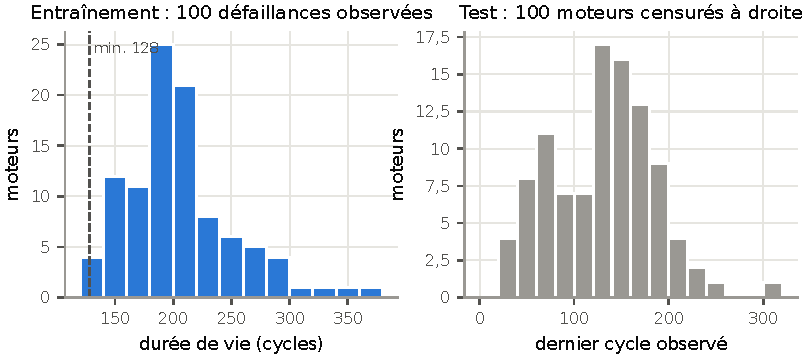
\includegraphics[width=1\linewidth]{figures/donnees_durees_de_vie.pdf}
\caption{Distribution des durées de vie des moteurs d'entraînement (gauche) et des durées observées des moteurs de test, censurées à droite (droite).}\label{fig:donnees_durees_de_vie}
\end{figure}

\section{Censure à droite}\label{sec:donnees-censure}

Pour l'analyse de fiabilité, les 200 moteurs forment une seule population. Les 100 moteurs d'entraînement fournissent des \textbf{durées de défaillance observées} (statut $\delta = 1$). Les 100 moteurs de test étaient encore en fonctionnement à leur dernier cycle observé : leur durée de vie est seulement connue pour être supérieure à ce cycle. Ce sont des \textbf{censures à droite} (statut $\delta = 0$). Le RUL réel des moteurs de test n'est pas utilisé dans l'analyse de fiabilité : il sert uniquement à évaluer les modèles de RUL, ce qui évite toute fuite d'information entre les deux parties de l'étude.

\section{Capteurs constants et analyse exploratoire}\label{sec:donnees-capteurs}

Le tableau~\ref{tab:donnees_capteurs} donne les statistiques des 21 capteurs et des réglages sur le jeu d'entraînement. Avec une seule condition opératoire, plusieurs capteurs ne varient pas ou presque : 7 capteurs présentent moins de 10 valeurs distinctes sur tout le jeu et sont écartés (s1, s5, s6, s10, s16, s18, s19). Les réglages opérationnels ne portent pas d'information de dégradation. Les autres capteurs dérivent progressivement au cours de la vie du moteur, comme le montre la figure~\ref{fig:donnees_signaux_moteur1} pour 6 d'entre eux : certains croissent (températures, pression statique en sortie du HPC), d'autres décroissent (pression en sortie du HPC, débits de refroidissement). Le bruit de mesure est important à l'échelle d'un cycle, d'où l'intérêt des moyennes glissantes.

\begin{table}[htbp]
\centering\small
\begin{adjustbox}{max width=\linewidth,center}
\begin{tabular}{llrrrl}
\toprule
Variable & Description & Moyenne & Écart-type & Valeurs distinctes & Statut \\
\midrule
set1 & Réglage opérationnel 1 & 0,000 & 0,002 & 158 & réglage \\
set2 & Réglage opérationnel 2 & 0,000 & 0,000 & 13 & réglage \\
set3 & Réglage opérationnel 3 & 100,000 & 0,000 & 1 & réglage \\
s1 & T2 — Température entrée fan (°R) & 518,670 & 0,000 & 1 & constant, écarté \\
s2 & T24 — Température sortie LPC (°R) & 642,681 & 0,500 & 310 & retenu \\
s3 & T30 — Température sortie HPC (°R) & 1\,590,523 & 6,131 & 3\,012 & retenu \\
s4 & T50 — Température sortie LPT (°R) & 1\,408,934 & 9,001 & 4\,051 & retenu \\
s5 & P2 — Pression entrée fan (psia) & 14,620 & 0,000 & 1 & constant, écarté \\
s6 & P15 — Pression bypass (psia) & 21,610 & 0,001 & 2 & constant, écarté \\
s7 & P30 — Pression sortie HPC (psia) & 553,368 & 0,885 & 513 & retenu \\
s8 & Nf — Vitesse physique fan (rpm) & 2\,388,097 & 0,071 & 53 & retenu \\
s9 & Nc — Vitesse physique core (rpm) & 9\,065,243 & 22,083 & 6\,403 & non retenu \\
s10 & epr — Rapport de pression moteur & 1,300 & 0,000 & 1 & constant, écarté \\
s11 & Ps30 — Pression statique sortie HPC (psia) & 47,541 & 0,267 & 159 & retenu \\
s12 & phi — Débit carburant / Ps30 & 521,414 & 0,738 & 427 & retenu \\
s13 & NRf — Vitesse corrigée fan (rpm) & 2\,388,096 & 0,072 & 56 & retenu \\
s14 & NRc — Vitesse corrigée core (rpm) & 8\,143,753 & 19,076 & 6\,078 & non retenu \\
s15 & BPR — Taux de dilution & 8,442 & 0,038 & 1\,918 & retenu \\
s16 & farB — Rapport carburant/air brûleur & 0,030 & 0,000 & 1 & constant, écarté \\
s17 & htBleed — Enthalpie de prélèvement & 393,211 & 1,549 & 13 & retenu \\
s18 & Nf\_dmd — Vitesse fan demandée & 2\,388,000 & 0,000 & 1 & constant, écarté \\
s19 & PCNfR\_dmd — Vitesse fan corrigée demandée & 100,000 & 0,000 & 1 & constant, écarté \\
s20 & W31 — Débit air refroidissement HPT & 38,816 & 0,181 & 120 & retenu \\
s21 & W32 — Débit air refroidissement LPT & 23,290 & 0,108 & 4\,745 & retenu \\
\bottomrule
\end{tabular}
\end{adjustbox}
\caption{Variables de FD001 (statistiques sur le jeu d'entraînement)}\label{tab:donnees_capteurs}
\end{table}

\begin{figure}[htbp]
\centering
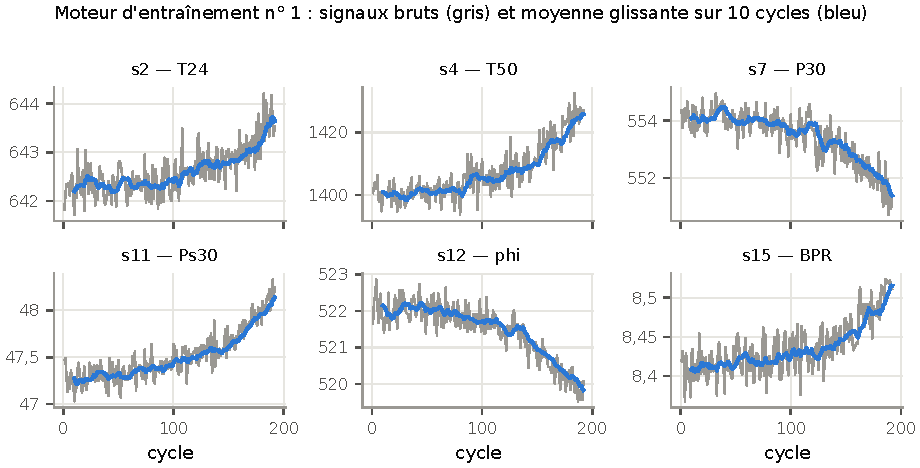
\includegraphics[width=1\linewidth]{figures/donnees_signaux_moteur1.pdf}
\caption{Signaux bruts de capteurs retenus pour le premier moteur d'entraînement et leur moyenne glissante : la dérive progressive vers la défaillance est visible malgré le bruit.}\label{fig:donnees_signaux_moteur1}
\end{figure}

\chapconclusion

Les données forment une population de 200 unités pour l'analyse de fiabilité, dont 100 durées censurées à droite. Aucune défaillance n'intervient avant 128 cycles, et 7 capteurs constants sont écartés. Le chapitre suivant présente les méthodes appliquées à ces données.
